\documentclass[prl,twocolumn,amsmath,amssymb,superscriptaddress]{revtex4-2}

\usepackage{graphicx}
\usepackage{verbatim}
\usepackage{braket}
\usepackage{epsfig}
\usepackage{epstopdf}
\usepackage{amsfonts}
\usepackage{amsthm}
\usepackage{amsmath}
\usepackage{amssymb}
\usepackage{color}
\usepackage[dvipsnames,svgnames,table]{xcolor}
\usepackage{hyperref}
\hypersetup{colorlinks=true,linkcolor=NavyBlue,citecolor=BrickRed,urlcolor=NavyBlue}
\usepackage{dsfont}
\usepackage{color}
\usepackage{grffile}
\usepackage{bm}
\usepackage{lipsum}
%end of packages

\begin{document}

\title{PHY180: Pendulum Project}
\author{Luyu Wu Vankerkwijk}
\date{\today}


\maketitle

\section{Introduction}
This paper investigates the non-linear behaviors of a pendulum, largely through experimental analysis, and correlates the findings to an offered linear model of the pendulum:

\begin{equation}
    \theta(t) = A_0e^{-t/\tau}cos\left(\frac{2\pi t}{T}+\phi_0\right)
    \label{eq:given}
\end{equation}

This equation (Wilson, 2025) defines the angle of the pendulum as a function of time, where $A_0$ and $\phi_0$ are initial conditions, and $\tau$ a constant damping factor.


Experiments were performed using a home-built pendulum, tracked using a high-speed camera. Data was processed to determine experimental relationships between amplitude-period, amplitude-damping, as well as length-period and length-damping were investigated.

\section{Experimental Methods}
The experimental setup consists of a 3 m string, wrapped around a cloth hanger attached to an overhang. A cloth hanger is used such that the string can be spooled to adjust the length of the pendulum.

The top of the string is bound tightly. At the bottom of the pendulum, a metal mass with a ring soldered onto it is tied. The mass of the pendulum blob is 54 grams while the full string's is roughly 2 grams. A strand length of $74.5 cm \pm 0.05 cm$ was used in trials where length was kept constant. Note that effective length is affected by other factors. A calibration ruler is placed on the hanger to provide a reference for tracker.

\begin{figure}[htb]
    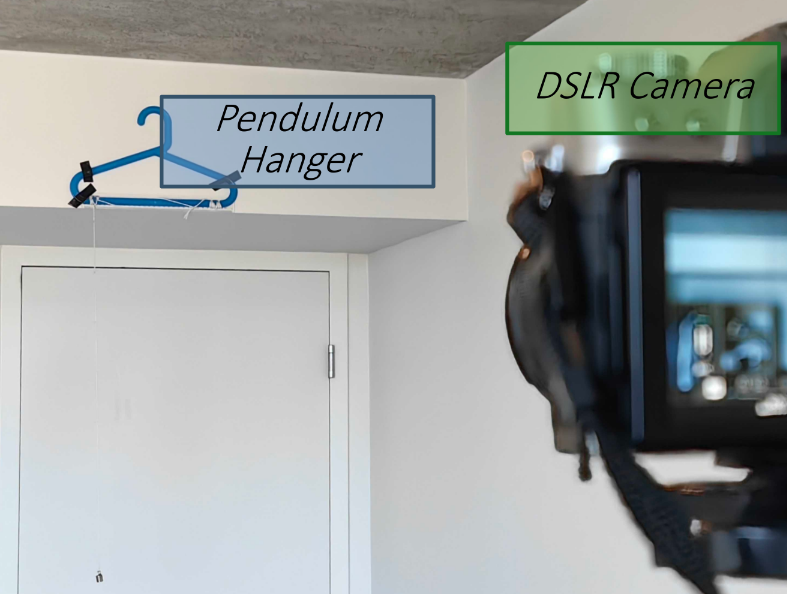
\includegraphics[width=0.68\linewidth]{setup.png}
    \caption{Picture of experimental setup. Pendulum blob is visible in the lower left corner.}
    \label{fig:experiment_setup}
\end{figure}

\newpage

The pendulum system was recorded from approximately 4 meters away (so as to minimize parallax) using a DSLR camera. A shutter speed of $1/1000$ and motion FPS of $60$ were used so as to minimize motion blurring, and maintain a high time resolution.

The pendulum was carefully released by hand. Drops where the pendulum moved significantly out-of-plane were removed (see Appendix B).



\begin{figure}[htb]
    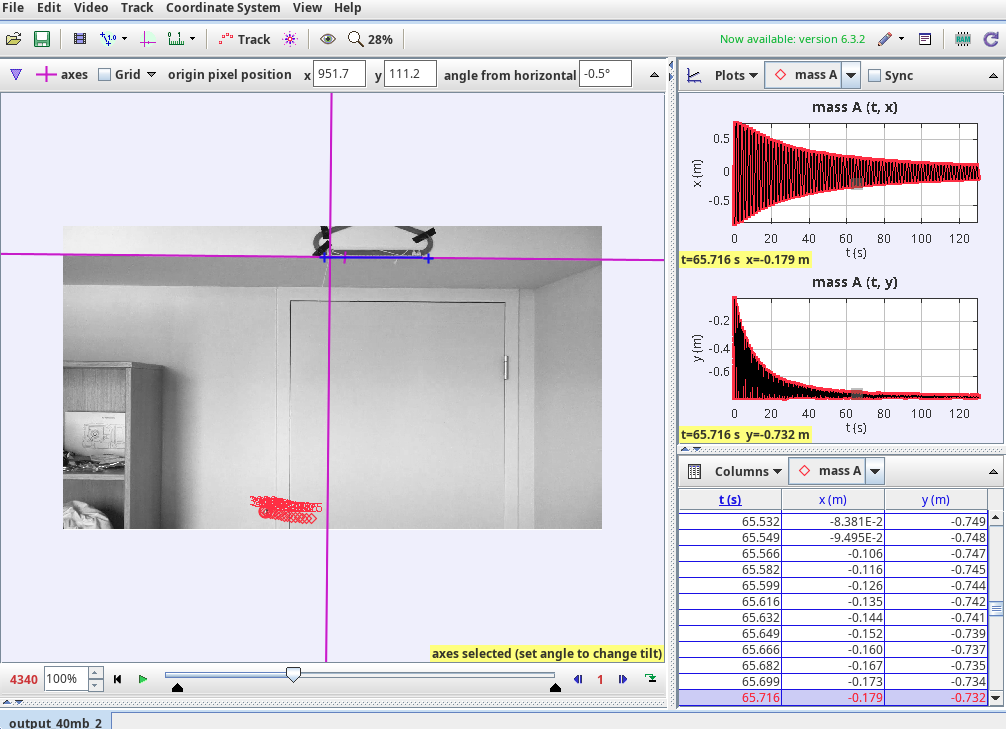
\includegraphics[width=0.7\linewidth]{tracker.png}
    \caption{OSP Tracker software used to obtain projected pendulum position as a function of time.}
    \label{fig:tracker}
\end{figure}

All data was processed in a custom Python script (see Appendix A). In processing the data, we assume that the motion of the pendulum is continuous in reality (for interpolation between points) so as to achieve better time resolution.

SciPy peak detection was performed to find local maxima. Periods were found by iterating through adjacent peak points and finding the time difference ($T_n=t_{n+1}-t_{n}$).

\begin{figure}[htb]
    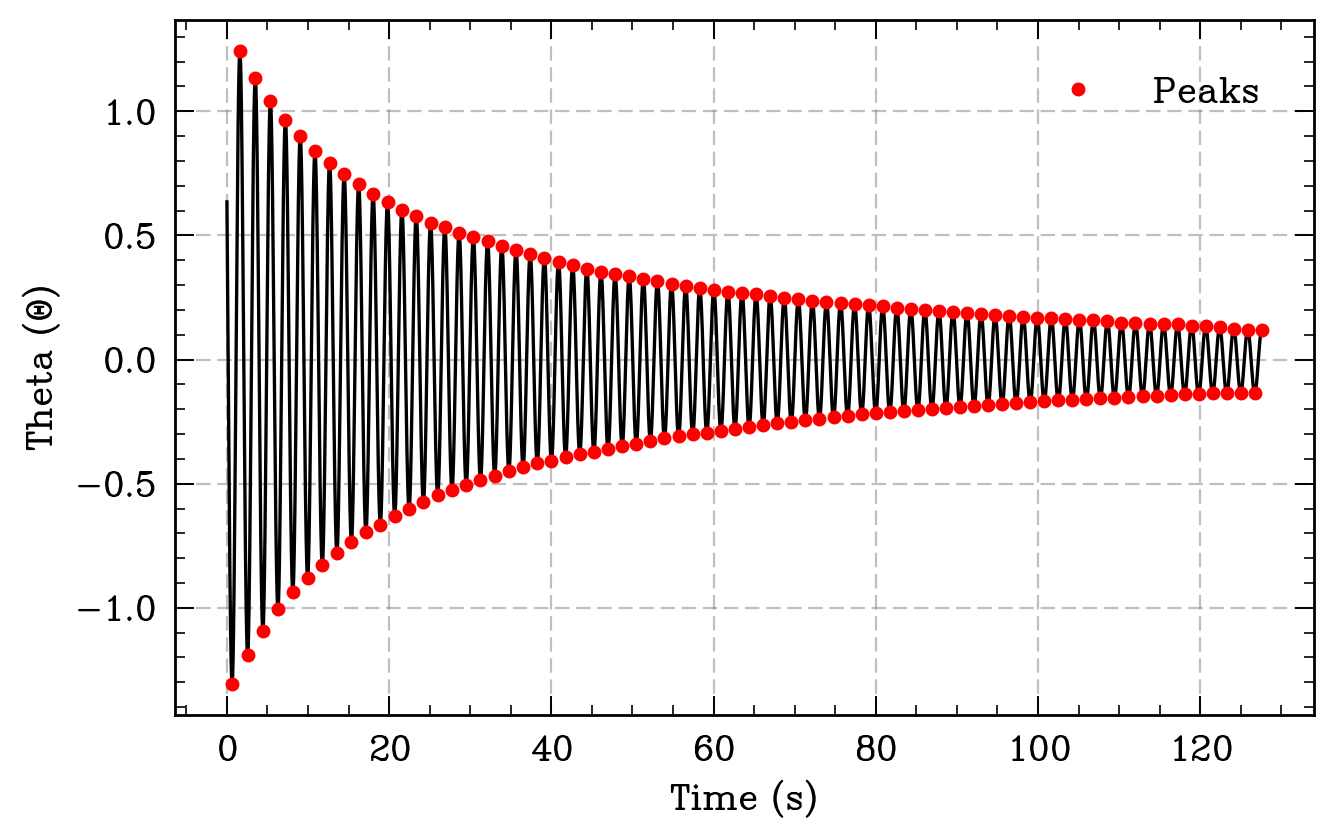
\includegraphics[width=0.8\linewidth]{angle_time.png}
    \caption{Plot of pendulum angle against time, along with detected peaks.}
    \label{fig:angle_time}
\end{figure}

\section{Analysis}


\subsection{Period Non-Linearity}

First, the period non-linearity of the system is analyzed. The governing equation given (eq. \ref{eq:given}) assumes the period of the system to be a constant.

By analyzing the relationship between amplitude and period, we can determine if this assumption is correct or not.

Based on the experimental data plotted in Fig. \ref{fig:amplitude-period}, the period is proportional to $A^2$ outside 2x the margin of error. Thus it is confident that the period is not constant for a given system (and instead varies with amplitude).


\begin{figure}[htb]
    \hspace{-20pt}
    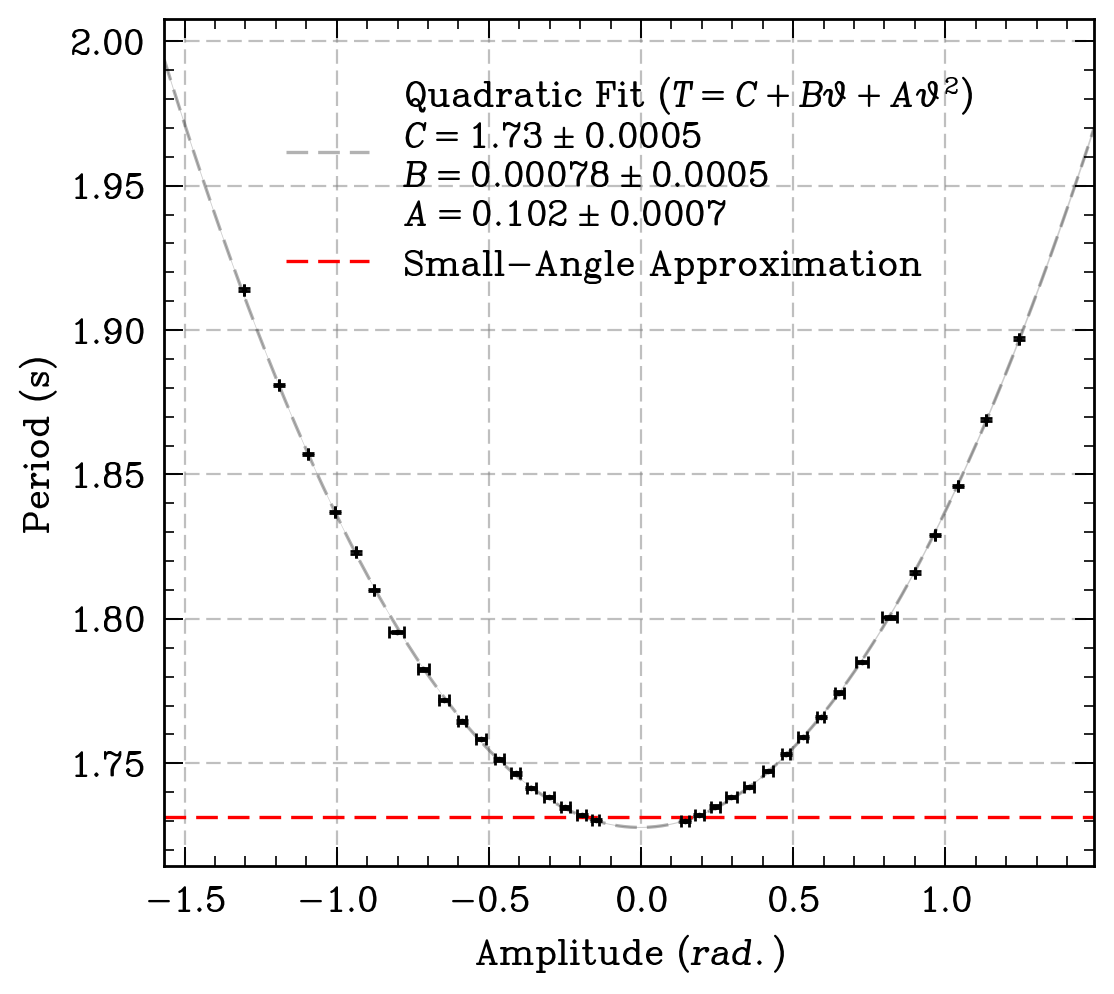
\includegraphics[width=0.85\linewidth]{amp_per_error_of_mean.png}
    \caption{Plot of pendulum period against oscillation amplitude. Datapoint errorbars are calculated as the standard deviation of the mean. $\theta$ as referenced in the legend is the transient amplitude of oscillation. Noticeably, the $B$ is experimentally 0, implying the period is not linearly (asymmetrically) dependent on amplitude.}
    \label{fig:amplitude-period}
\end{figure}

Subsequent trials are done in amplitude regimes where the change in period is experimentally zero. This correlates to $A\in[-0.15,0.15]$, where we the linear approximation is within error for all values (see Fig. \ref{fig:small-angles}).

\begin{figure}[htb]
    \hspace{-20pt}
    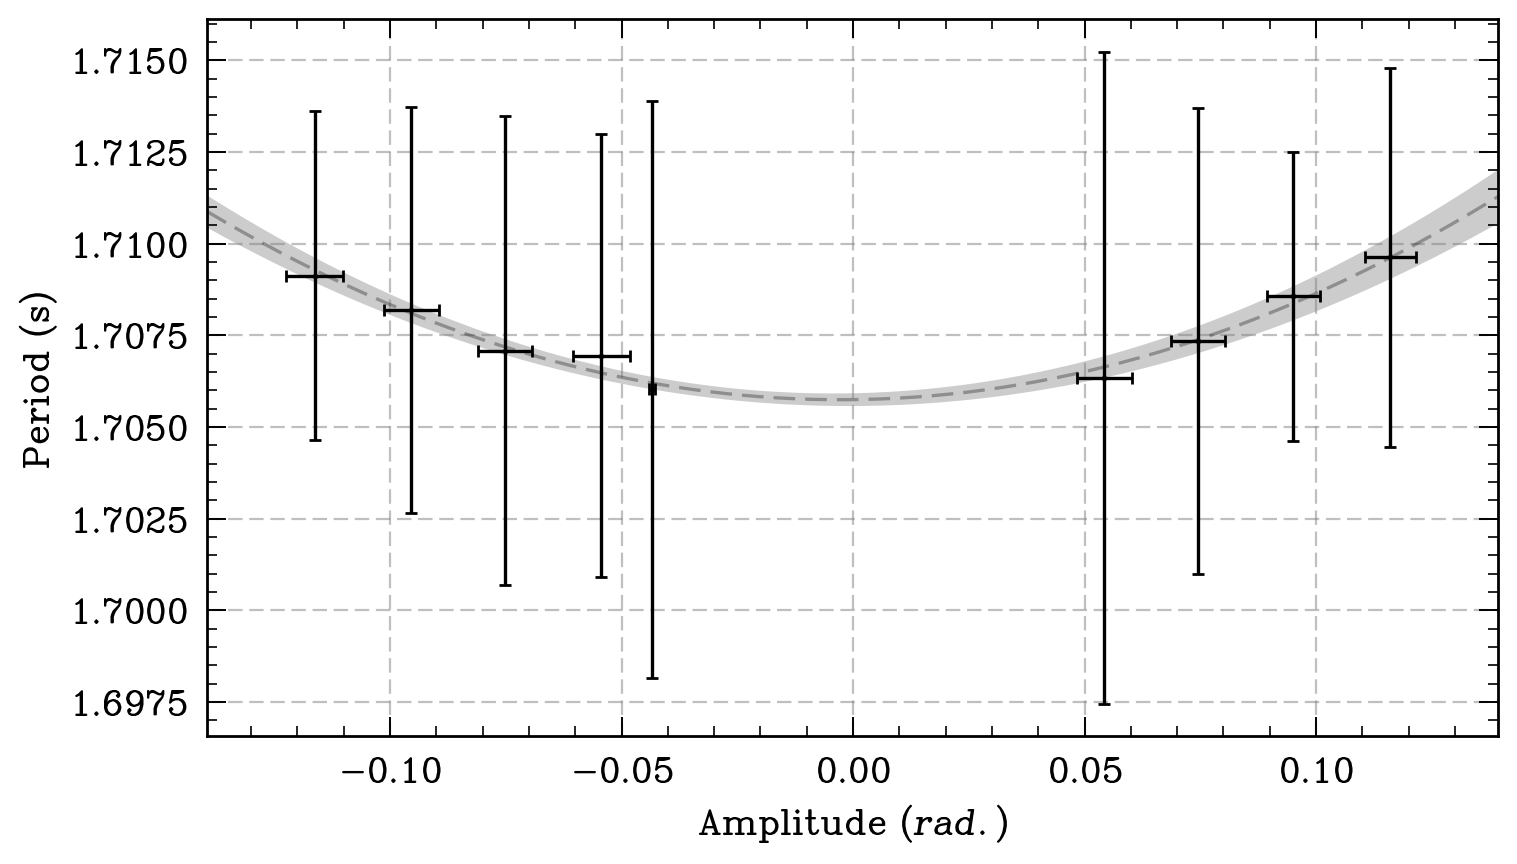
\includegraphics[width=0.8\linewidth]{Q-factor-smallangleusage.png}
    \caption{Plot of pendulum period against oscillation amplitude at small angles. Independent data of Fig. \ref{fig:angle_time}, \ref{fig:amplitude-period}.}
    \label{fig:small-angles}
\end{figure}

\subsection{Damping Factor}

Investigating the damping is a critical part of understanding the pendulum's motion. We can define a dimensionless Q factor, where the Q-factor defines the ratio of energy loss in relation in a radian of a cycle.

Q-factor can be most easily found using either an exponential fit ($Q=\pi\frac{\tau}{T}$). The real pendulum system experiences various damping forces (Couloumb, viscous, and turbulent largely), some of which vary as amplitude decreases. This causes the Q-factor to be non-constant across time in our system as visible in Figure \ref{fig:decay}.

\begin{figure}[htb]
    \hspace{-20pt}
    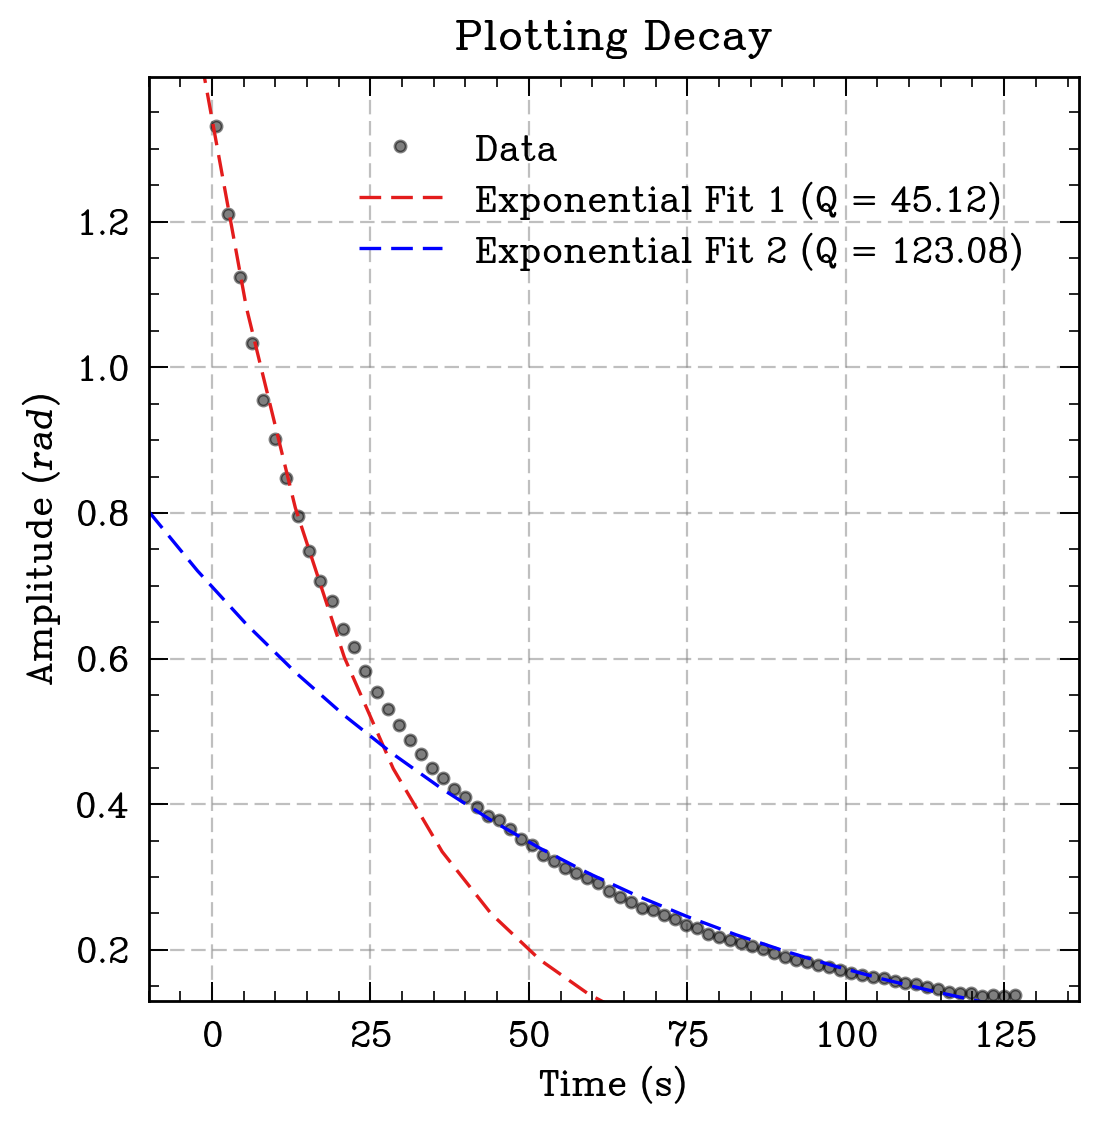
\includegraphics[width=0.8\linewidth]{decay.png}
    \caption{Plot of pendulum amplitude against time. Two $Q$ numbers are found for different regions where $t_1\in[0s,25s], t_2\in[75s,125s]$. This shows $Q$ to be dependent on amplitude.}
    \label{fig:decay}
\end{figure}

If Q is instead found at low-amplitudes, where the small-angle approximation is more appropriate, we observe a much better fit (Fig. \ref{fig:decay_small_angle}).
\begin{figure}[htb]
    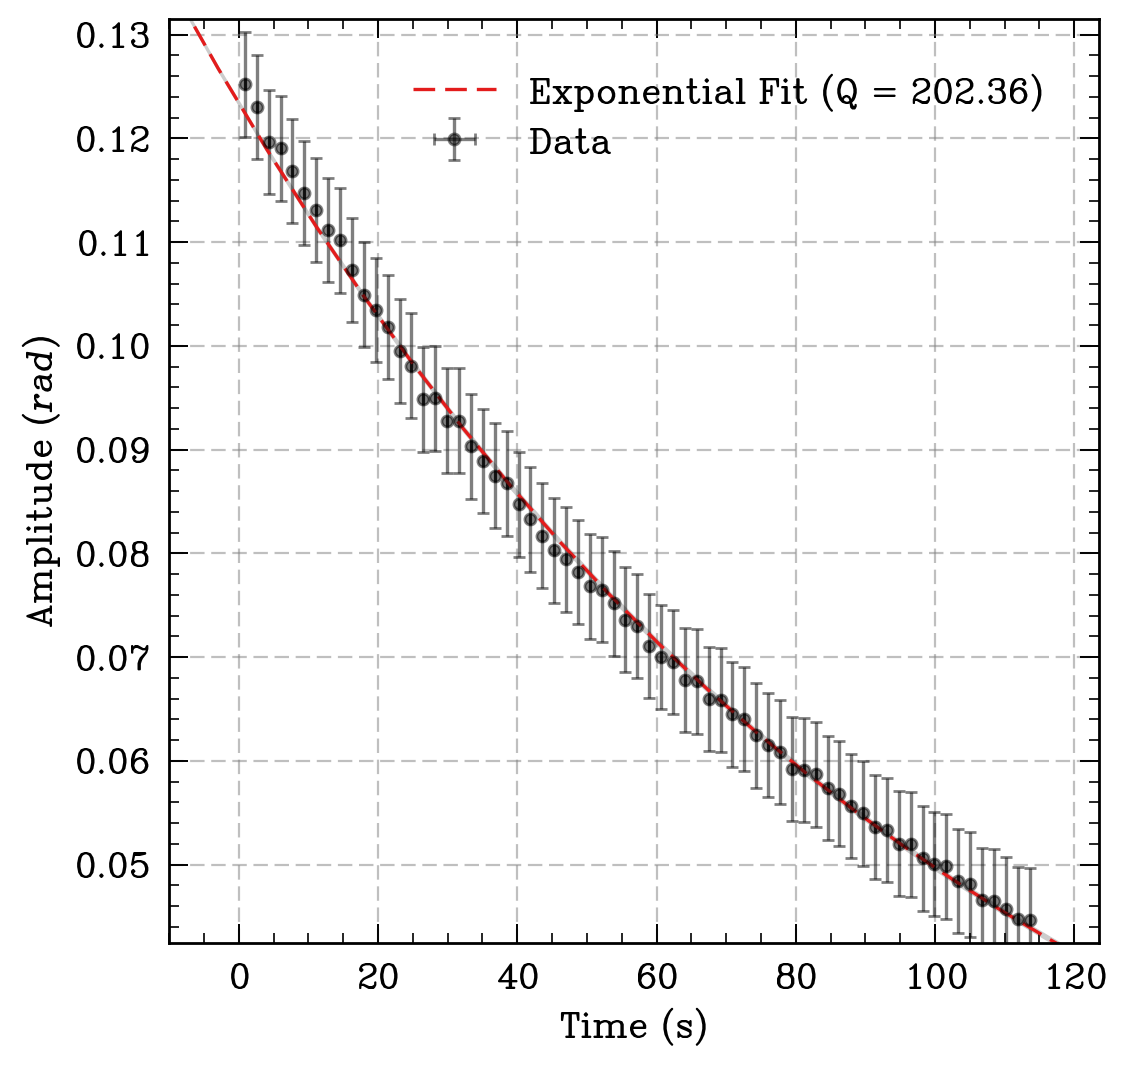
\includegraphics[width=0.8\linewidth]{low_angle_q.png}
    \caption{Plot of pendulum amplitude against time. Since the range of the amplitudes is smaller in this case, an exponential fit is much better.}
    \label{fig:decay_small_angle}
\end{figure}

The Q-factor is found to be $202\pm0.9$ using the fit $\tau$ factor. Error is found through the fit error.

Alternatively, the Q-factor can be found by counting the oscillations it takes for the system to dampen to $A_0(e^{-\pi/C})$, then multiplying that number by $C$ (Wilson, 2025). A visualization of this method can be seen in Fig. \ref{fig:count_q}.

\begin{figure}[htb]
    \hspace{-20pt}
    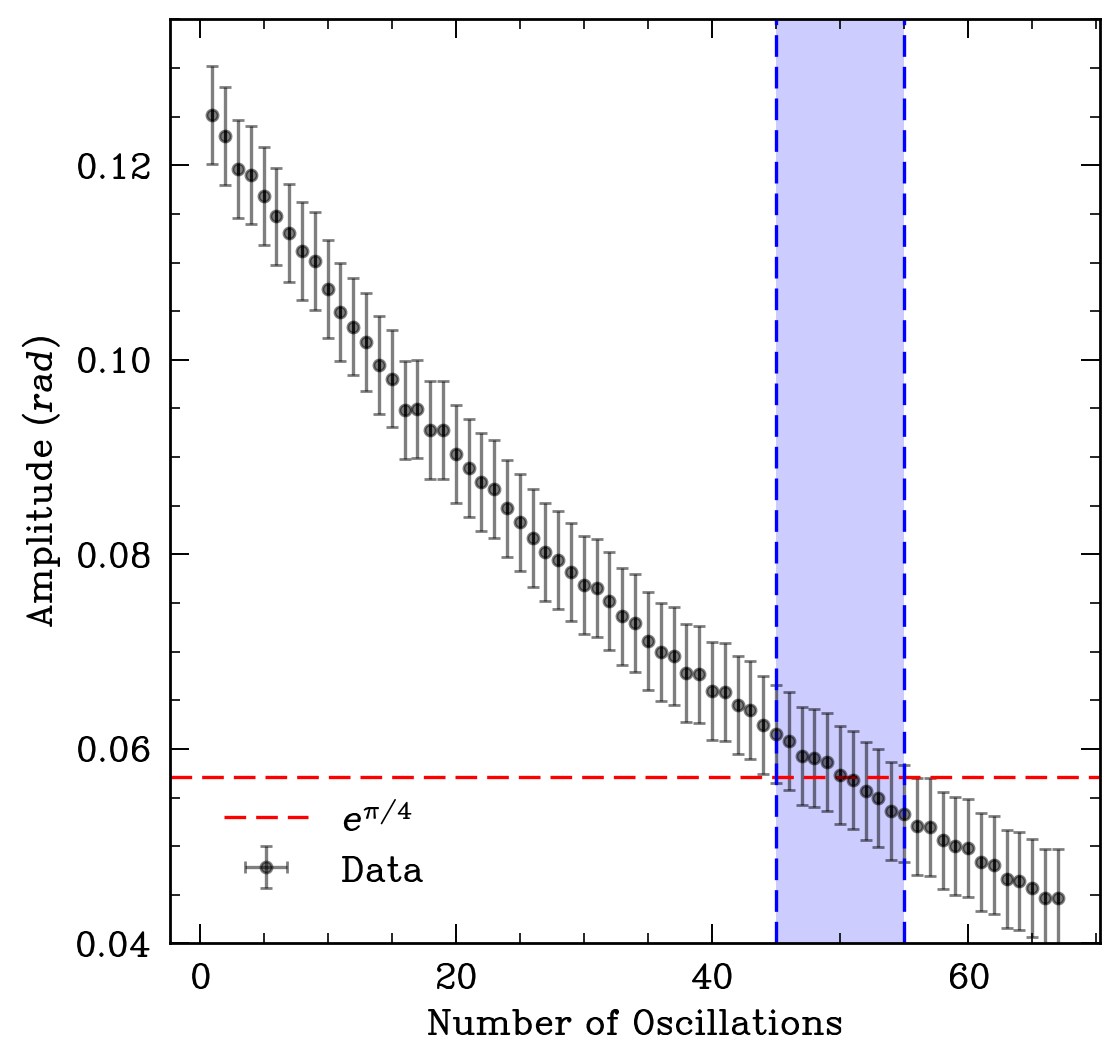
\includegraphics[width=0.8\linewidth]{count_decay.png}
    \caption{Amplitude of oscillation vs. oscillation number. Oscillation counting method is used to find number of oscillations before amplitude reaches $e^{-\pi/4}$ (the red line). The blue range represents amplitude peaks which intersect the red line. Here, the number of oscillations is found to be $50\pm5$, thus Q-factor is found to be $200\pm20$.}
    \label{fig:count_q}
\end{figure}

Using oscillation counting, the Q-factor is found to be $200\pm20$, where the larger error as compared to the exponential fit can be explained by the more discretized methodology.

Importantly, the Q-factors found by the two different methods are highly similar and within error of each other ($202\pm0.9$ and $200\pm20$ respectively). This implies an accurate Q-value characterization of the system within the low-amplitude regime.

\vspace{64pt}
\section{Determining Uncertainties}

The uncertainty is selected between Type A and Type B depending on which is larger. In this section, the derivation of Type B errors are explained, given they are not clear in certain scenarios such when using camera tracking.

The Type B uncertainty of the time of measurement (which propagates to period) is negligible as the camera's shutter speed is $1/1000$. Error seen in period-amplitude is thus calculated through Type A. This noise likely sources from amplitude Type B uncertainty, which through peak detection, translates into noise in period data.

The uncertainty for the amplitude of the pendulum seen in Figure 6 and 7 are determined through the Type B uncertainty of the amplitude. The width of the pendulum (of which Tracker may not always select the centre of) causes measurement errors. It is calculated as $\epsilon = \frac{w}{2(l)}$ for a 68\% confidence. Measurement of the width was done in Tracker to calibrate error to the data (see Appendix C). This error may be minimized by using an indicator (e.g. black dot) instead of tracking the whole blob.

\section{Conclusion}
In this report, various aspects of the pendulum's motion were investigated in relation to the offered closed-form equation.

Firstly, a experimental setup consisting of a metal-blob pendulum and DSLR camera was engineered. Precautions were taken to ensure error due to string mass, parallax, and out-of-plane oscillations were minimized.

Secondly, using experimental data, it is proven that $T$ and $\tau$ are not constant as the equation suggests, but instead heavily dependent on the amplitude of oscillation (see Fig. \ref{fig:amplitude-period}, \ref{fig:decay}).

By analyzing oscillations at small angles (within error of a constant period), we are able to characterize the Q-factor of the system ($202\pm0.9$). This value was verified using the manual oscillation counting method as well.


\onecolumngrid

\newpage
\section{Appendix}

\subsection{A. Processing Code}

All of the code (as well as video files and tracked CSV) used for this project is open-sourced on GitHub, and can be accessed here: \href{https://github.com/luyu-wu/Pendulum-Project}{https://github.com/luyu-wu/Pendulum-Project}.

All code is written by me, with credit to modules NumPy, MatPlotLib, and SciPy.

\subsection{B. Out-of-plane Oscillations}

In the case that this report investigates, the pendulum has 2 degrees of freedom ($\phi, \theta$). Since the plane that our camera projects is not sensitive to $\phi$, the resultant $\theta$ found is dependent on $\phi$ through $cos(\phi)x_{pendulum} = x_{observed}$.

Thus, tracking the pendulum using a camera, care must be taken to avoid the pendulum going out of plane (in other words, keep $\phi$ at a desirable constant value).

A solution to this is using purely the $y$-tracked values, as these are not dependent on $\phi$ (ignoring parallax, which is not important in our setup).
However, at small angles, these are significantly harder to track due to vanishing derivative $\frac{dcos(\theta)}{d\theta}$ as $\theta \Rightarrow 0$.


\begin{figure}[htb]
    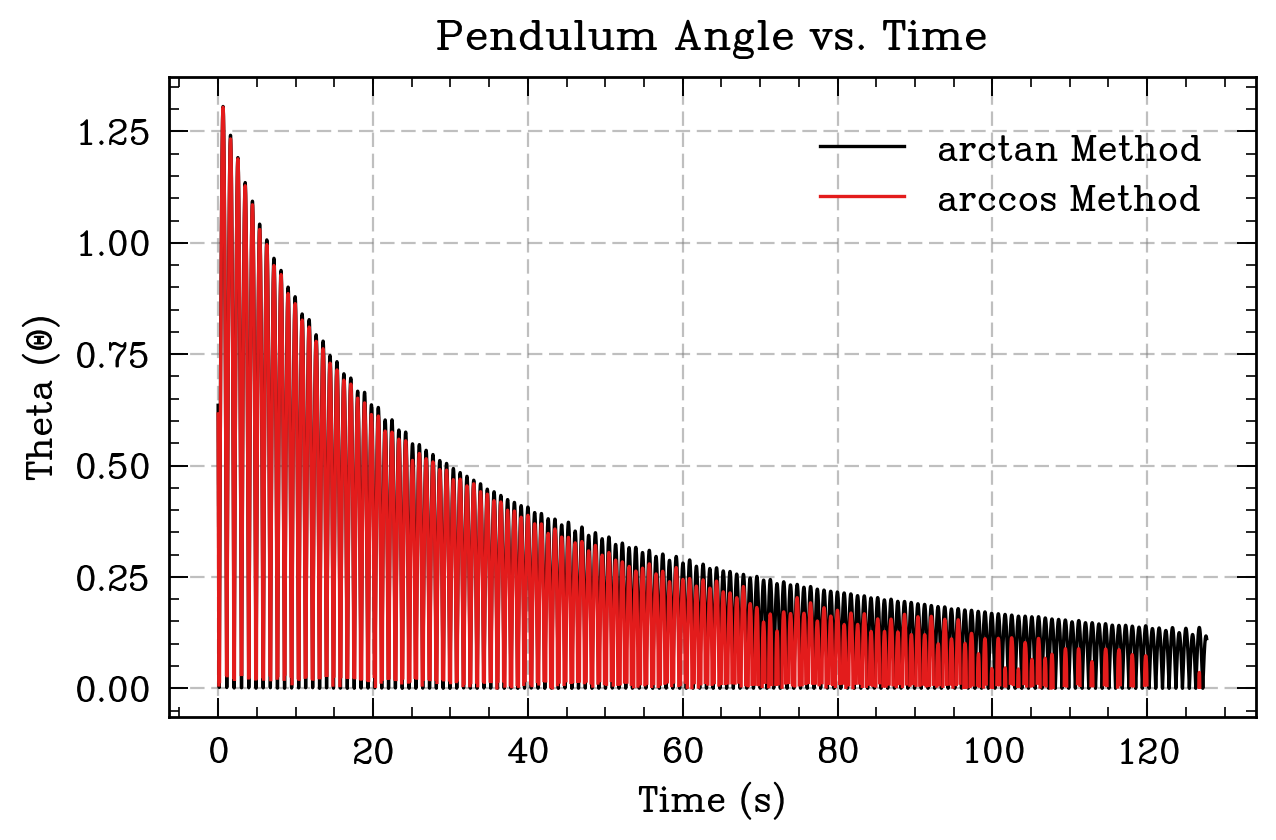
\includegraphics[width=0.4\linewidth]{out-of-plane.png}
    \label{fig:out-of-plane}
    \caption{This graph shows the differences in results between tracking with $\phi$ dependence and without. Note that the reason no negative $\theta$ exists is because that would require us to know $\phi$, something not possible purely from $y$.}
\end{figure}

\subsection{C. Measurement Uncertainty of Amplitude}

As mentioned in \textbf{Determining Uncertainties}, the Type B uncertainty of the pendulum's position must be determined. To find this, the maximum width of the pendulum in the Tracker software is found. This is at the bottom of its motion, where motion blur is greatest. The uncertainty is then found through this via $\epsilon = \frac{w}{2(l)}$ so as to represent a 68\% confidence interval. Note that this assumes tracker has a uniform selection density across the pendulum body, which implies this error is overestimated. This process can be seen in Fig. \ref{fig:body}.
\begin{figure}[htb]
    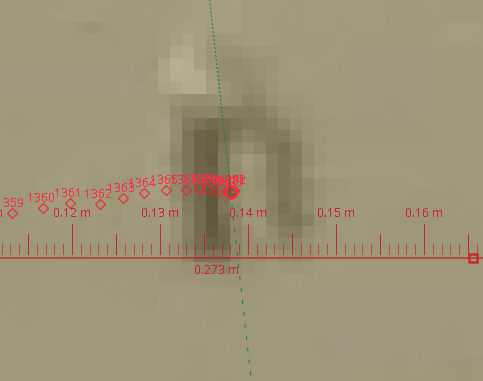
\includegraphics[width=0.2\linewidth]{pendulum-body.png}
    \caption{The measurement of the width of the pendulum is shown here. The length is propagated from the calibration stick.}
    \label{fig:body}
\end{figure}

\newpage

\section{References}

Wilson, Brian, “PHY180 Pendulum Project”, from
\href{https://q.utoronto.ca/courses/411727/files/39071655?module_item_id=7122439}{q.utoronto.ca}, 2025.


\subsection{AI Statement}

No form of AI was used in assisting the writing of this lab.

\end{document}
